\documentclass[a4j,11pt]{jarticle}
\usepackage{amsmath}
\usepackage{amssymb}
\usepackage{wrapfig}
\usepackage{mathrsfs}
\usepackage{cases}
\usepackage{braket}
\usepackage{verbatim}
\usepackage{latexsym}
\usepackage[dvipdfmx]{graphicx}

%--余白の設定
\setlength{\topmargin}{20mm}
\addtolength{\topmargin}{-1in}
\setlength{\oddsidemargin}{20mm}
\addtolength{\oddsidemargin}{-1in}
\setlength{\evensidemargin}{15mm}
\addtolength{\evensidemargin}{-1in}
\setlength{\textwidth}{170mm}
\setlength{\textheight}{254mm}
\setlength{\headsep}{0mm}
\setlength{\headheight}{0mm}
\setlength{\topskip}{0mm}

\usepackage{listings, jlisting}
\renewcommand{\lstlistingname}{リスト}
\lstset{language=C++,%
        basicstyle=\footnotesize,%
        commentstyle=\textit,%
        classoffset=1,%
        keywordstyle=\bfseries,%
	frame=tRBl,framesep=5pt,%
	showstringspaces=false,%
        numbers=left,stepnumber=1,numberstyle=\footnotesize
	}%

\makeatletter
  \def\thefootnote{\ifnum\c@footnote>\z@\leavevmode\lower.5ex%
      \hbox{$^{\@arabic\c@footnote)}$}\fi}
\makeatother

\title{PRML輪講 第一回}
\author{}
\date{\today}

 \def\v#1{\mbox{\boldmath $#1$}}
 \def\d#1#2{\frac{d #1}{d #2}}
 \def\dd#1#2{\frac{d^2 #1}{d #2 ^2}}
 \def\dn#1#2#3{\frac{d^#1 #2}{d #3 ^#1}}
 \def\pd#1#2{\frac{\partial #1}{\partial #2}}
 \def\pdd#1#2{\frac{\partial^2 #1}{\partial #2 ^2}}
 \def\pdn#1#2#3{\frac{\partial^#1 #2}{\partial #3 ^#1}}
 
 \def\j#1{\v{j}(\v{x}^{(#1)})}
 \def\x#1{\v{x}^{(#1)}}
 
 \def\tjx{\v{\tilde{\jmath}}(\v{x})}
 \def\tjxd{\v{\tilde{\jmath}}(\v{x'})}
 
 \def\deL{\mathscr{L}}

\begin{document}
%\twocolumn[
%\maketitle
%
%\renewcommand\thefootnote{\roman{footnote}}
%]

\maketitle

\section*{1章 序論}
\begin{itemize}
	\item 結局何をしたいのか\\
		$\rightarrow$ \textbf{データに内在するパターンを明らかにしたい}
	\item 例 (手書き文字の認識)(イメージ図\ref{fig:learning1}参照)\\
		\begin{figure}[htbp]
			\centering
			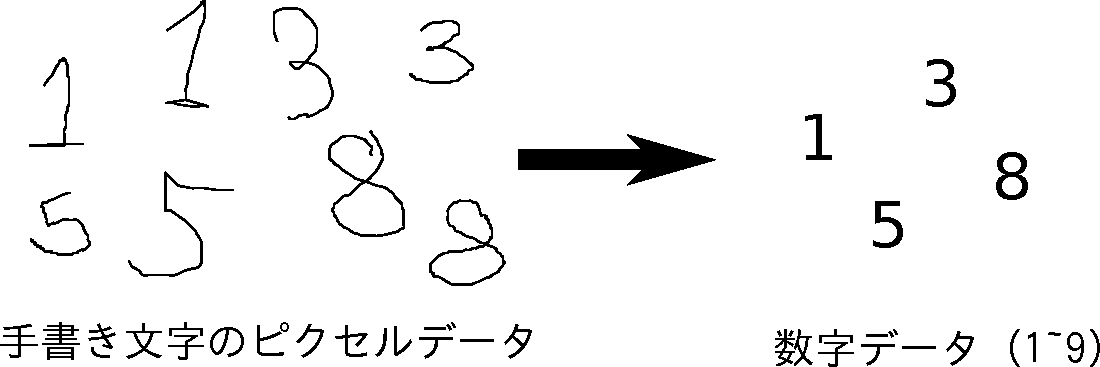
\includegraphics[width=10cm]{learning1.pdf}
			\caption{文字認識のイメージ図}
			\label{fig:learning1}
		\end{figure}
		\begin{itemize}
			\item 入力: $\v{x}$ (ピクセルを表現するような実数値ベクトル)\\
				出力: 0から9までの数字
			\item \v{x}を与えると0から9までの数字を出してくれるような機械を作りたい
		\end{itemize}
	\item 機械学習的なアプローチ
		\begin{itemize}
			\item 調節可能なパラメータを持つモデルを用意
			\item $N$個の手書き文字データ (\textbf{訓練集合})$\{\v{x}_1 \cdots \v{x}_N\}$とそれぞれの文字データに対応する数字 (\textbf{目標ベクトル}) $\v{t}$を用いて、パラメータを調整する。
			\item 最終的に画像$\v{x}$を入力すると対応する何らかの数字$\v{y}$を返してくれる関数$\v{y}(\v{x})$が生成される。
			\item 訓練集合にはなかった数字データ$\v{x}$ (\textbf{テスト集合})に対しても対応する数字を推測することができるようになる。
		\end{itemize}
	\item テスト集合に対してどれぐらい正確に数字を判定することができるか$\rightarrow$ \textbf{汎化性能}
		\begin{itemize}
			\item いくら訓練集合に対して正確に数字を当てることができたとしてもテスト集合でダメダメな結果であれば意味がない。 (過学習)
		\end{itemize}
	\item \textbf{\underline{目標: 汎化性能を向上させたい}}
	\item その他のトピック
		\begin{itemize}
			\item 本来は入力変数を扱いやすい形に変換しておく$\rightarrow$ 前処理
			\item 訓練データが入力変数$\v{x}$のみで目標値がないタイプの問題もある$\rightarrow$ 教師なし学習 (クラスタリングや密度推定などの問題)
			\item 与えられた状況で報酬を最大にする行動を学習 $\rightarrow$ 強化学習
		\end{itemize}
	\item まずはわかりやすい例(回帰問題)から初めて概念を説明することにする
\end{itemize}
\section*{1.1 多項式線形フィッティング}
\begin{itemize}
	\item 問題設定
		\begin{itemize}
			\item 訓練集合としてN個の観測値を並べた入力$\v{\mathrm{x}} = (x_1 \ldots x_N)^{\mathrm{T}}$と出力$\v{\mathrm{t}} = (t_1 \ldots t_N)^{\mathrm{T}}$を用意
			\item 出力は$\sin(2\pi x)$ にノイズ ($\xi$)を加えて生成するが、具体的な関数形$\sin(2\pi x)$ は事前に知らされていないものとする
				\begin{align}
					t_n = \sin(2\pi x_n) + \xi
				\end{align}
			\item これらのデータでモデルを訓練させることで、新たなテスト集合として$x$が与えられても、それに対する出力$t$が正しく推測されるようにしたい (汎化性能の向上)
		\end{itemize}
	\item まずはナイーブなアプローチ (多項式フィッティング)を考えてみる
		\begin{align}
			y(x, \v{w}) = \sum_{j=0}^{M}w_jx^{j}
		\end{align}
		\begin{itemize}
			\item 調節可能なパラメータは$\v{w}$と$M$
		\end{itemize}
	\item 単純に二乗和誤差$E(\v{w})$を最小にするようにパラメータ$\v{w}$を求めることを考える (ただの最小二乗法)
		\footnote{一見単純なことを延々とやっているようにも見えるが、後半でこのアプローチが確率を用いた枠組みで説明できることがわかる}
		\begin{align}
			E(\v{w}) = \frac{1}{2}\sum_{n=1}^{N}\{y(x_n, \v{w})-t_n\}^2 
		\end{align}
\end{itemize}
\subsection*{演習1.1の解}
$E(\v{w})$を最小にするような$\v{w}$を求めるため、誤差関数を$w_i$で微分することを考えると、
\begin{align*}
	\pd{}{w_i}E(\v{w}) &= \sum_{n=1}^{N}\{y(x_n, \v{w})-t_n\}\cdot x_n^{i} \nonumber \\
			&= \sum_{n=1}^{N}\sum_{j=0}^{M}w_j x_n^{j}x_n^{i} - \sum_{n=1}^{N}t_n x_n^{i} = 0
\end{align*}
整理して
\begin{align}
	\sum_{j=0}^{M}\left(\sum_{n=1}^N x_n^{i+j}\right)w_j = \sum_{n=1}^{N}t_nx_n^j
\end{align}
となるから、これより$\v{w}$が一意に決まることがわかる。
\begin{itemize}
		\item まだパラメーターとして多項式の次数$M$が残っている
		\item $M$を増やせば増やすほどモデルを複雑にでき、誤差関数を0に近づけることができる
			\begin{itemize}
				\item 特に、データ数と同じ数に$M$を設定すると誤差関数は必ず0となる
			\end{itemize}
		\item \textbf{誤差関数を小さくしさえすればそれでOKなのか?}
			\begin{itemize}
				\item 次数$M$を大きくしすぎると与えられたデータに無理やり合わせたような結果になり、明らかに$\sin(2\pi x)$を表現していない $\rightarrow$ \textbf{過学習}
				\item 過学習が起きないように (まずは場当たり的に?)工夫する必要がある
			\end{itemize}
		\item 過学習の回避方法
			\begin{itemize}
				\item 訓練集合を増やすことで過学習は起こりにくくなる (教科書図1.6)
					\begin{itemize}
						\item (訓練集合に対応してモデルの複雑さを変えるのはいかがなものか)
					\end{itemize}
				\item 過学習が起きるとき、$\v{w}$のノルムが大きくなる傾向があるため、これをペナルティ項を用いて抑える $\rightarrow$ \textbf{正則化}
					\footnote{この手法も後で確率を用いた定式化ができる。}
					\begin{align}
						\tilde{E}(\v{w}) = \frac{1}{2}\sum_{n=1}^{N}\{y(x_n, \v{w})-t_n\}^2+\frac{\lambda}{2}|\v{w}|^2
					\end{align}
				\item この場合の誤差関数を最小にする$\v{w}$も、前と同じように1つに定まる。
			\end{itemize}
\end{itemize}
\subsection*{演習1.2の解}
同じように誤差関数を$w_i$で微分すると、
\begin{align*}
	\pd{}{w_i}\tilde{E}(\v{w}) &= \sum_{n=1}^{N}\{y(x_n, \v{w})-t_n\}\cdot x_n^{i}+\lambda w_i  = 0\nonumber \\
\end{align*}
整理して
\begin{align}
	\sum_{j=0}^{M}\left(\sum_{n=1}^N x_n^{i+j}+\lambda \delta_{ij}\right)w_j = \sum_{n=1}^{N}t_nx_n^j
\end{align}
となる。
\begin{itemize}
	\item $M$や$\lambda$についてはどう考慮すべきか
		\begin{itemize}
			\item 得られているデータを訓練集合と、それとは別にチェックを行う用の\textbf{確認集合}に分ける
			\item 訓練に使えるデータが減ってしまうデメリットがある
		\end{itemize}
	\item 次の節から今までの概念を\textbf{確率}の観点で説明することを考える
\end{itemize}
\newpage
\section*{1.2 確率論}
\begin{itemize}
	\item 確率の基本法則 (そこまで詳しく行う必要はないと思うので簡単に紹介)
		\begin{itemize}
			\item 加法定理
				\begin{align}
					p(X) = \sum_{Y}p(X,Y)
				\end{align}
			\item 乗法定理
				\begin{align}
					p(X,Y) = p(X|Y)p(Y)
				\end{align}
		\end{itemize}
	\item 同時確率の対称性$P(X,Y)=P(Y,X)$を用いることで、
		\begin{align}
			P(Y|X)P(X) = P(X|Y)P(Y)
		\end{align}
		であることから、\textbf{ベイズの定理}
		\begin{align}
			P(Y|X) = \frac{P(X|Y)P(Y)}{P(X)}
		\end{align}
		が成り立つ。
		\begin{itemize}
			\item 条件付き確率の変数 (ここでは$X$と$Y$)をひっくり返すことができる。
		\end{itemize}
	\item \textbf{頻度主義} (ざっくりいうと従来の確率の扱い)と\textbf{ベイズ主義} (ざっくりいうと新しい確率の見方)の違い
		\begin{itemize}
			\item \textbf{\underline{頻度主義}}\\
				観測されたデータは\textbf{「神のみぞ知る唯一無二の真のモデル」から発生したものの1つ}であると考える。つまり真のモデルはただ1つだけであり、データは確率的に変動すると考える。データをいっぱい取りまくれば (観測しまくれば)それだけ真値に近づくことができると考える。
			\item \textbf{\underline{ベイズ主義}}\\
				\textbf{唯一無二の真のモデルなど存在しない。データが全て}である。データを取ることにより (観測することにより)真値の"確率分布"をベイズの定理を用いて逐次更新していく。ここで言う"確率"とは"信念の度合い"のようなものを指す。\footnote{確率が高い$\to$おそらくそれっぽいだろう、確率が低い$\to$たぶんこれではないだろう、といった具合。合格率xx割みたいな使いかたに近い。}
				\begin{itemize}
					\item ベイズ主義の適用例 (教科書p15参照)
					\item オレンジを得たという情報を得ることにより、箱の色がどっちであるかという確率がベイズの定理により更新される。$P(赤い色の箱を選んだ確率) \to ベイズの定理 \to P(\textbf{箱からオレンジを取り出した時点での、}赤い色の箱を選んだ確率)$
				\end{itemize}
			\item 要するに、\textbf{頻度主義では真値が定数でデータが確率変数、ベイズ主義ではデータが定数で真値が確率変数}
			\item 前の多項式フィッティングの例で考えてみると、ベイズの定理で次のように表せる、
				\begin{align}
					P(\v{w}|\v{\mathrm{t}}) = \frac{P(\v{\mathrm{t}|\v{w}})P(\v{w})}{P(\v{\mathrm{t}})}
				\end{align}
				ここで
				\begin{align}
					P(\v{w}) &\cdots (まだ情報が与えられてない時点での)パラメータの確率 (信念の度合い) \\
					P(\v{\mathrm{t}|\v{w}}) &\cdots パラメータ\v{w}を固定した際の観測データ\v{\mathrm{t}}の起こりやすさ \\
					P(\v{w}|\v{\mathrm{t}}) &\cdots (観測データが与えられたという条件の元での)パラメータの確率 (信念の度合い)
				\end{align}
			\item $P(\v{w})$を事前確率、$P(\v{\mathrm{t}|\v{w}})$を尤度関数、$P(\v{w}|\v{\mathrm{t}})$を事後確率と呼ぶ。
			\item ベイズの定理を用いることで、$\v{w}$が与えられたときのデータ$\v{\mathrm{t}}$の分布から、この2つをひっくり返した、データ$\v{\mathrm{t}}$が与えられたときの$\v{w}$の分布を評価できるという強みがある。
		\end{itemize}
	\item そもそもやりたかったことは何か $\to$ パラメータ$\v{w}$の推定
	\item 頻度主義で広く用いられる手法 $\to$ \textbf{最尤推定} 
		\begin{itemize}
			\item $P(\v{\mathrm{t}|\v{w}})$を最大にするような$\v{w}$を選んでくる。
			\item 手元にあるデータを最も実現しそうな (最も尤もらしい)パラメータ$\v{w}$を決める操作
		\end{itemize}
	\item この後、尤度関数をガウス分布と仮定することで (前に見た)最小二乗法と最尤法とのつながりが見えることを示す。
	\item ガウス分布 ($\mu$: 平均、$\sigma^2$: 分散)
		\begin{align}
			\mathcal{N}(x|\mu, \sigma^2) = \frac{1}{\sqrt{2\pi \sigma^2}}e^{-\frac{1}{2\sigma^2}(x-\mu)^2}
		\end{align}
	\item 特に多変量ガウス分布の場合 ($D$次元の場合) (\v{\Sigma}: 共分散行列)
		\footnote{規格化因子は共分散行列を対角化することで求められる。}
		\begin{align}
			\mathcal{N}(\v{x}|\v{\mu}, \v{\Sigma}) = \frac{1}{(2\pi)^{D/2}}\frac{1}{|\v{\Sigma}|^{1/2}} \exp\left\{-\frac{1}{2}(\v{x}-\v{\mu})^{\mathrm{T}}\v{\Sigma}^{-1}(\v{x}-\v{\mu})\right\}
		\end{align}
	\item $N$個の観測データ$\v{\mathrm{x}}_{\mathrm{tr}}=(x_1, \ldots, x_N)^{\mathrm{T}}$がガウス分布から独立に生成されるとすると、(i.i.d)
		\begin{align}
			p(\v{\mathrm{x}}_{\mathrm{tr}}|\mu, \sigma^2) = \prod_{n=1}^{N}\mathcal{N}(x_n | \mu, \sigma^2)
		\end{align}
	\item 最尤法 $\to$ $p(\v{\mathrm{x}}_{\mathrm{tr}}|\mu, \sigma^2)$を$\v{\mathrm{x}}_{\mathrm{tr}}|$について最大化するような$\mu$と$\sigma^2$を求める問題
		\begin{itemize}
			\item 解いてみると
				\begin{align}
					\mu_{\mathrm{ML}} &= \frac{1}{N}\sum_{n=1}^{N}x_n \\
					\sigma_{\mathrm{ML}}^2 &= \frac{1}{N}\sum_{n=1}^{N}(x_n-\mu_{\mathrm{ML}})^2
				\end{align}
			\item $\sigma_{\mathrm{ML}}^2$の期待値が$\sigma^2$に一致せず、$(N-1)/N$倍に縮小されてしまう。 $\to$ 最尤法による過学習の問題と関連
		\end{itemize}
	\item 曲線フィッティングとの関係
		\begin{itemize}
			\item 二乗和誤差の最小化 $\to$ 尤度関数がガウス分布 (平均$y(x, \v{w})$, 分散$\beta^{-1}$)で与えられたと仮定したときの最尤法と同じ
				\begin{itemize}
					\item 推定された値$\v{w}_{\mathrm{ML}}、\v{\beta}_{\mathrm{ML}}$を用いて新たな$x$が与えられたときの$t$の分布を推定できる
				\end{itemize}
			\item 正則化も含めた場合の最小化 $\to$ 事前分布を導入した際の\textbf{事後確率の最大化 (MAP)}と定式化できる
		\end{itemize}

	\item $\v{\mathrm{ML}}$を点推定するだけでなく、$\v{w}$のすべての値で積分することにより、よりベイズ的な扱いをして予測分布を求める。

\end{itemize}


\end{document}
